% SOURCE: edit-harness/results/frame_a/cells/cell_*_real_MIX_{A,B,C}_*.json + results/D3_benefit_predictor_eval.json
% !TEX encoding = UTF-8 Unicode
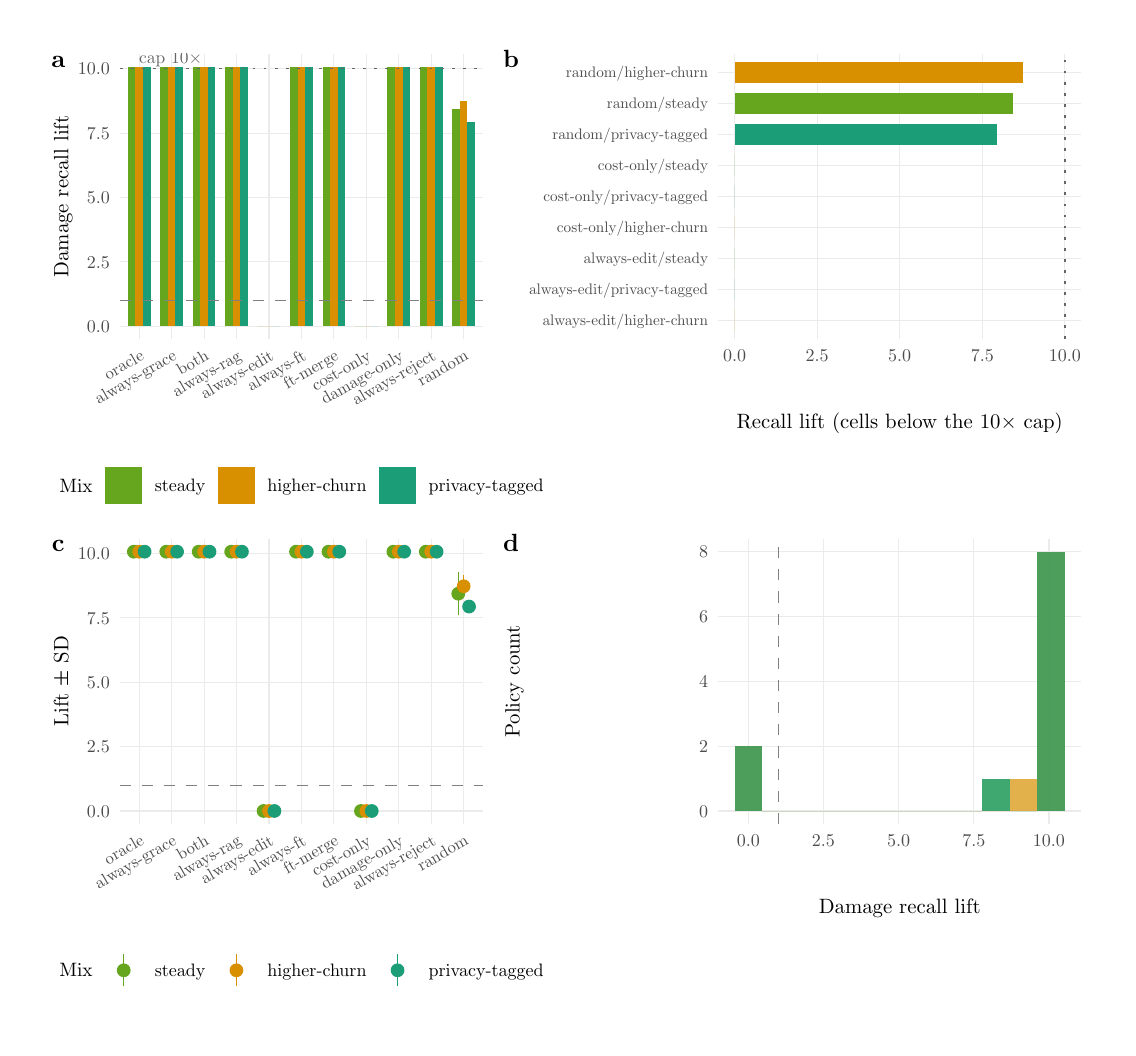
\begin{tikzpicture}[x=1pt,y=1pt]
\definecolor{fillColor}{RGB}{255,255,255}
\path[use as bounding box,fill=fillColor,fill opacity=0.00] (0,0) rectangle (390.26,361.35);
\begin{scope}
\path[clip] (  0.00,  0.00) rectangle (390.26,361.35);
\definecolor{drawColor}{RGB}{255,255,255}
\definecolor{fillColor}{RGB}{255,255,255}

\path[draw=drawColor,line width= 0.6pt,line join=round,line cap=round,fill=fillColor] (  0.00,  0.00) rectangle (390.26,361.35);
\end{scope}
\begin{scope}
\path[clip] (  5.50,180.68) rectangle (168.58,355.85);
\definecolor{fillColor}{RGB}{255,255,255}

\path[fill=fillColor] (  5.50,180.68) rectangle (168.58,355.85);
\end{scope}
\begin{scope}
\path[clip] (168.58,180.68) rectangle (384.76,355.85);
\definecolor{fillColor}{RGB}{255,255,255}

\path[fill=fillColor] (168.58,180.68) rectangle (384.76,355.85);
\end{scope}
\begin{scope}
\path[clip] (  5.50,  5.50) rectangle (168.58,180.67);
\definecolor{fillColor}{RGB}{255,255,255}

\path[fill=fillColor] (  5.50,  5.50) rectangle (168.58,180.67);
\end{scope}
\begin{scope}
\path[clip] (168.58,  5.50) rectangle (384.76,180.67);
\definecolor{fillColor}{RGB}{255,255,255}

\path[fill=fillColor] (168.58,  5.50) rectangle (384.76,180.67);
\end{scope}
\begin{scope}
\path[clip] ( 33.28,248.80) rectangle (164.58,351.85);
\definecolor{drawColor}{gray}{0.92}

\path[draw=drawColor,line width= 0.4pt,line join=round] ( 33.28,253.48) --
	(164.58,253.48);

\path[draw=drawColor,line width= 0.4pt,line join=round] ( 33.28,276.74) --
	(164.58,276.74);

\path[draw=drawColor,line width= 0.4pt,line join=round] ( 33.28,299.99) --
	(164.58,299.99);

\path[draw=drawColor,line width= 0.4pt,line join=round] ( 33.28,323.25) --
	(164.58,323.25);

\path[draw=drawColor,line width= 0.4pt,line join=round] ( 33.28,346.51) --
	(164.58,346.51);

\path[draw=drawColor,line width= 0.4pt,line join=round] ( 40.31,248.80) --
	( 40.31,351.85);

\path[draw=drawColor,line width= 0.4pt,line join=round] ( 52.03,248.80) --
	( 52.03,351.85);

\path[draw=drawColor,line width= 0.4pt,line join=round] ( 63.76,248.80) --
	( 63.76,351.85);

\path[draw=drawColor,line width= 0.4pt,line join=round] ( 75.48,248.80) --
	( 75.48,351.85);

\path[draw=drawColor,line width= 0.4pt,line join=round] ( 87.20,248.80) --
	( 87.20,351.85);

\path[draw=drawColor,line width= 0.4pt,line join=round] ( 98.93,248.80) --
	( 98.93,351.85);

\path[draw=drawColor,line width= 0.4pt,line join=round] (110.65,248.80) --
	(110.65,351.85);

\path[draw=drawColor,line width= 0.4pt,line join=round] (122.37,248.80) --
	(122.37,351.85);

\path[draw=drawColor,line width= 0.4pt,line join=round] (134.10,248.80) --
	(134.10,351.85);

\path[draw=drawColor,line width= 0.4pt,line join=round] (145.82,248.80) --
	(145.82,351.85);

\path[draw=drawColor,line width= 0.4pt,line join=round] (157.54,248.80) --
	(157.54,351.85);
\definecolor{fillColor}{RGB}{102,166,31}

\path[fill=fillColor] ( 36.21,253.48) rectangle ( 38.94,347.17);

\path[fill=fillColor] ( 47.93,253.48) rectangle ( 50.67,347.17);

\path[fill=fillColor] ( 59.65,253.48) rectangle ( 62.39,347.17);

\path[fill=fillColor] ( 71.38,253.48) rectangle ( 74.11,347.17);

\path[fill=fillColor] ( 83.10,253.48) rectangle ( 85.84,253.48);

\path[fill=fillColor] ( 94.82,253.48) rectangle ( 97.56,347.17);

\path[fill=fillColor] (106.55,253.48) rectangle (109.28,347.17);

\path[fill=fillColor] (118.27,253.48) rectangle (121.01,253.48);

\path[fill=fillColor] (129.99,253.48) rectangle (132.73,347.17);

\path[fill=fillColor] (141.72,253.48) rectangle (144.45,347.17);

\path[fill=fillColor] (153.44,253.48) rectangle (156.18,332.00);
\definecolor{fillColor}{RGB}{216,144,0}

\path[fill=fillColor] ( 38.94,253.48) rectangle ( 41.68,347.17);

\path[fill=fillColor] ( 50.67,253.48) rectangle ( 53.40,347.17);

\path[fill=fillColor] ( 62.39,253.48) rectangle ( 65.12,347.17);

\path[fill=fillColor] ( 74.11,253.48) rectangle ( 76.85,347.17);

\path[fill=fillColor] ( 85.84,253.48) rectangle ( 88.57,253.48);

\path[fill=fillColor] ( 97.56,253.48) rectangle (100.29,347.17);

\path[fill=fillColor] (109.28,253.48) rectangle (112.02,347.17);

\path[fill=fillColor] (121.01,253.48) rectangle (123.74,253.48);

\path[fill=fillColor] (132.73,253.48) rectangle (135.46,347.17);

\path[fill=fillColor] (144.45,253.48) rectangle (147.19,347.17);

\path[fill=fillColor] (156.18,253.48) rectangle (158.91,334.67);
\definecolor{fillColor}{RGB}{27,158,119}

\path[fill=fillColor] ( 41.68,253.48) rectangle ( 44.41,347.17);

\path[fill=fillColor] ( 53.40,253.48) rectangle ( 56.14,347.17);

\path[fill=fillColor] ( 65.12,253.48) rectangle ( 67.86,347.17);

\path[fill=fillColor] ( 76.85,253.48) rectangle ( 79.58,347.17);

\path[fill=fillColor] ( 88.57,253.48) rectangle ( 91.31,253.48);

\path[fill=fillColor] (100.29,253.48) rectangle (103.03,347.17);

\path[fill=fillColor] (112.02,253.48) rectangle (114.75,347.17);

\path[fill=fillColor] (123.74,253.48) rectangle (126.48,253.48);

\path[fill=fillColor] (135.46,253.48) rectangle (138.20,347.17);

\path[fill=fillColor] (147.19,253.48) rectangle (149.92,347.17);

\path[fill=fillColor] (158.91,253.48) rectangle (161.65,327.35);
\definecolor{drawColor}{gray}{0.50}

\path[draw=drawColor,line width= 0.5pt,dash pattern=on 4pt off 4pt ,line join=round] ( 33.28,262.78) -- (164.58,262.78);
\definecolor{drawColor}{gray}{0.40}

\path[draw=drawColor,line width= 0.5pt,dash pattern=on 1pt off 3pt ,line join=round] ( 33.28,346.51) -- (164.58,346.51);

\node[text=drawColor,anchor=base west,inner sep=0pt, outer sep=0pt, scale=  0.63] at ( 40.31,348.23) {cap $10\times$};
\end{scope}
\begin{scope}
\path[clip] (  0.00,  0.00) rectangle (390.26,361.35);
\definecolor{drawColor}{gray}{0.30}

\node[text=drawColor,anchor=base east,inner sep=0pt, outer sep=0pt, scale=  0.65] at ( 29.68,251.24) {0.0};

\node[text=drawColor,anchor=base east,inner sep=0pt, outer sep=0pt, scale=  0.65] at ( 29.68,274.50) {2.5};

\node[text=drawColor,anchor=base east,inner sep=0pt, outer sep=0pt, scale=  0.65] at ( 29.68,297.76) {5.0};

\node[text=drawColor,anchor=base east,inner sep=0pt, outer sep=0pt, scale=  0.65] at ( 29.68,321.01) {7.5};

\node[text=drawColor,anchor=base east,inner sep=0pt, outer sep=0pt, scale=  0.65] at ( 29.68,344.27) {10.0};
\end{scope}
\begin{scope}
\path[clip] (  0.00,  0.00) rectangle (390.26,361.35);
\definecolor{drawColor}{gray}{0.30}

\node[text=drawColor,rotate= 30.00,anchor=base east,inner sep=0pt, outer sep=0pt, scale=  0.60] at ( 42.38,241.62) {oracle};

\node[text=drawColor,rotate= 30.00,anchor=base east,inner sep=0pt, outer sep=0pt, scale=  0.60] at ( 54.10,241.62) {always-grace};

\node[text=drawColor,rotate= 30.00,anchor=base east,inner sep=0pt, outer sep=0pt, scale=  0.60] at ( 65.82,241.62) {both};

\node[text=drawColor,rotate= 30.00,anchor=base east,inner sep=0pt, outer sep=0pt, scale=  0.60] at ( 77.55,241.62) {always-rag};

\node[text=drawColor,rotate= 30.00,anchor=base east,inner sep=0pt, outer sep=0pt, scale=  0.60] at ( 89.27,241.62) {always-edit};

\node[text=drawColor,rotate= 30.00,anchor=base east,inner sep=0pt, outer sep=0pt, scale=  0.60] at (100.99,241.62) {always-ft};

\node[text=drawColor,rotate= 30.00,anchor=base east,inner sep=0pt, outer sep=0pt, scale=  0.60] at (112.72,241.62) {ft-merge};

\node[text=drawColor,rotate= 30.00,anchor=base east,inner sep=0pt, outer sep=0pt, scale=  0.60] at (124.44,241.62) {cost-only};

\node[text=drawColor,rotate= 30.00,anchor=base east,inner sep=0pt, outer sep=0pt, scale=  0.60] at (136.16,241.62) {damage-only};

\node[text=drawColor,rotate= 30.00,anchor=base east,inner sep=0pt, outer sep=0pt, scale=  0.60] at (147.89,241.62) {always-reject};

\node[text=drawColor,rotate= 30.00,anchor=base east,inner sep=0pt, outer sep=0pt, scale=  0.60] at (159.61,241.62) {random};
\end{scope}
\begin{scope}
\path[clip] (  0.00,  0.00) rectangle (390.26,361.35);
\definecolor{drawColor}{RGB}{0,0,0}

\node[text=drawColor,rotate= 90.00,anchor=base,inner sep=0pt, outer sep=0pt, scale=  0.75] at ( 14.67,300.32) {Damage recall lift};
\end{scope}
\begin{scope}
\path[clip] (  0.00,  0.00) rectangle (390.26,361.35);
\definecolor{drawColor}{RGB}{0,0,0}

\node[text=drawColor,anchor=base west,inner sep=0pt, outer sep=0pt, scale=  0.70] at ( 11.43,193.49) {Mix};
\end{scope}
\begin{scope}
\path[clip] (  0.00,  0.00) rectangle (390.26,361.35);
\definecolor{fillColor}{RGB}{102,166,31}

\path[fill=fillColor] ( 28.00,189.19) rectangle ( 41.42,202.61);
\end{scope}
\begin{scope}
\path[clip] (  0.00,  0.00) rectangle (390.26,361.35);
\definecolor{fillColor}{RGB}{216,144,0}

\path[fill=fillColor] ( 68.72,189.19) rectangle ( 82.14,202.61);
\end{scope}
\begin{scope}
\path[clip] (  0.00,  0.00) rectangle (390.26,361.35);
\definecolor{fillColor}{RGB}{27,158,119}

\path[fill=fillColor] (126.95,189.19) rectangle (140.37,202.61);
\end{scope}
\begin{scope}
\path[clip] (  0.00,  0.00) rectangle (390.26,361.35);
\definecolor{drawColor}{RGB}{0,0,0}

\node[text=drawColor,anchor=base west,inner sep=0pt, outer sep=0pt, scale=  0.65] at ( 45.94,193.66) {steady};
\end{scope}
\begin{scope}
\path[clip] (  0.00,  0.00) rectangle (390.26,361.35);
\definecolor{drawColor}{RGB}{0,0,0}

\node[text=drawColor,anchor=base west,inner sep=0pt, outer sep=0pt, scale=  0.65] at ( 86.66,193.66) {higher-churn};
\end{scope}
\begin{scope}
\path[clip] (  0.00,  0.00) rectangle (390.26,361.35);
\definecolor{drawColor}{RGB}{0,0,0}

\node[text=drawColor,anchor=base west,inner sep=0pt, outer sep=0pt, scale=  0.65] at (144.89,193.66) {privacy-tagged};
\end{scope}
\begin{scope}
\path[clip] (  0.00,  0.00) rectangle (390.26,361.35);
\definecolor{drawColor}{RGB}{0,0,0}

\node[text=drawColor,anchor=base,inner sep=0pt, outer sep=0pt, scale=  0.90] at ( 11.05,347.07) {\bfseries a};
\end{scope}
\begin{scope}
\path[clip] (249.46,248.80) rectangle (380.76,351.85);
\definecolor{drawColor}{gray}{0.92}

\path[draw=drawColor,line width= 0.4pt,line join=round] (249.46,255.52) --
	(380.76,255.52);

\path[draw=drawColor,line width= 0.4pt,line join=round] (249.46,266.72) --
	(380.76,266.72);

\path[draw=drawColor,line width= 0.4pt,line join=round] (249.46,277.92) --
	(380.76,277.92);

\path[draw=drawColor,line width= 0.4pt,line join=round] (249.46,289.12) --
	(380.76,289.12);

\path[draw=drawColor,line width= 0.4pt,line join=round] (249.46,300.32) --
	(380.76,300.32);

\path[draw=drawColor,line width= 0.4pt,line join=round] (249.46,311.52) --
	(380.76,311.52);

\path[draw=drawColor,line width= 0.4pt,line join=round] (249.46,322.73) --
	(380.76,322.73);

\path[draw=drawColor,line width= 0.4pt,line join=round] (249.46,333.93) --
	(380.76,333.93);

\path[draw=drawColor,line width= 0.4pt,line join=round] (249.46,345.13) --
	(380.76,345.13);

\path[draw=drawColor,line width= 0.4pt,line join=round] (255.42,248.80) --
	(255.42,351.85);

\path[draw=drawColor,line width= 0.4pt,line join=round] (285.27,248.80) --
	(285.27,351.85);

\path[draw=drawColor,line width= 0.4pt,line join=round] (315.11,248.80) --
	(315.11,351.85);

\path[draw=drawColor,line width= 0.4pt,line join=round] (344.95,248.80) --
	(344.95,351.85);

\path[draw=drawColor,line width= 0.4pt,line join=round] (374.79,248.80) --
	(374.79,351.85);
\definecolor{fillColor}{RGB}{102,166,31}

\path[fill=fillColor] (255.42,274.00) rectangle (255.42,281.84);

\path[fill=fillColor] (255.42,307.60) rectangle (255.42,315.44);
\definecolor{fillColor}{RGB}{216,144,0}

\path[fill=fillColor] (255.42,251.60) rectangle (255.42,259.44);

\path[fill=fillColor] (255.42,285.20) rectangle (255.42,293.04);
\definecolor{fillColor}{RGB}{27,158,119}

\path[fill=fillColor] (255.42,262.80) rectangle (255.42,270.64);

\path[fill=fillColor] (255.42,296.40) rectangle (255.42,304.24);

\path[fill=fillColor] (255.42,318.81) rectangle (350.20,326.65);
\definecolor{fillColor}{RGB}{102,166,31}

\path[fill=fillColor] (255.42,330.01) rectangle (356.17,337.85);
\definecolor{fillColor}{RGB}{216,144,0}

\path[fill=fillColor] (255.42,341.21) rectangle (359.60,349.05);
\definecolor{drawColor}{gray}{0.40}

\path[draw=drawColor,line width= 0.5pt,dash pattern=on 1pt off 3pt ,line join=round] (374.79,248.80) -- (374.79,351.85);
\end{scope}
\begin{scope}
\path[clip] (  0.00,  0.00) rectangle (390.26,361.35);
\definecolor{drawColor}{gray}{0.30}

\node[text=drawColor,anchor=base east,inner sep=0pt, outer sep=0pt, scale=  0.55] at (245.86,253.62) {always-edit/higher-churn};

\node[text=drawColor,anchor=base east,inner sep=0pt, outer sep=0pt, scale=  0.55] at (245.86,264.82) {always-edit/privacy-tagged};

\node[text=drawColor,anchor=base east,inner sep=0pt, outer sep=0pt, scale=  0.55] at (245.86,276.03) {always-edit/steady};

\node[text=drawColor,anchor=base east,inner sep=0pt, outer sep=0pt, scale=  0.55] at (245.86,287.23) {cost-only/higher-churn};

\node[text=drawColor,anchor=base east,inner sep=0pt, outer sep=0pt, scale=  0.55] at (245.86,298.43) {cost-only/privacy-tagged};

\node[text=drawColor,anchor=base east,inner sep=0pt, outer sep=0pt, scale=  0.55] at (245.86,309.63) {cost-only/steady};

\node[text=drawColor,anchor=base east,inner sep=0pt, outer sep=0pt, scale=  0.55] at (245.86,320.83) {random/privacy-tagged};

\node[text=drawColor,anchor=base east,inner sep=0pt, outer sep=0pt, scale=  0.55] at (245.86,332.03) {random/steady};

\node[text=drawColor,anchor=base east,inner sep=0pt, outer sep=0pt, scale=  0.55] at (245.86,343.24) {random/higher-churn};
\end{scope}
\begin{scope}
\path[clip] (  0.00,  0.00) rectangle (390.26,361.35);
\definecolor{drawColor}{gray}{0.30}

\node[text=drawColor,anchor=base,inner sep=0pt, outer sep=0pt, scale=  0.65] at (255.42,240.72) {0.0};

\node[text=drawColor,anchor=base,inner sep=0pt, outer sep=0pt, scale=  0.65] at (285.27,240.72) {2.5};

\node[text=drawColor,anchor=base,inner sep=0pt, outer sep=0pt, scale=  0.65] at (315.11,240.72) {5.0};

\node[text=drawColor,anchor=base,inner sep=0pt, outer sep=0pt, scale=  0.65] at (344.95,240.72) {7.5};

\node[text=drawColor,anchor=base,inner sep=0pt, outer sep=0pt, scale=  0.65] at (374.79,240.72) {10.0};
\end{scope}
\begin{scope}
\path[clip] (  0.00,  0.00) rectangle (390.26,361.35);
\definecolor{drawColor}{RGB}{0,0,0}

\node[text=drawColor,anchor=base,inner sep=0pt, outer sep=0pt, scale=  0.75] at (315.11,216.59) {Recall lift (cells below the $10\times$ cap)};
\end{scope}
\begin{scope}
\path[clip] (  0.00,  0.00) rectangle (390.26,361.35);
\definecolor{drawColor}{RGB}{0,0,0}

\node[text=drawColor,anchor=base,inner sep=0pt, outer sep=0pt, scale=  0.90] at (174.66,347.07) {\bfseries b};
\end{scope}
\begin{scope}
\path[clip] ( 33.28, 73.62) rectangle (164.58,176.68);
\definecolor{drawColor}{gray}{0.92}

\path[draw=drawColor,line width= 0.4pt,line join=round] ( 33.28, 78.30) --
	(164.58, 78.30);

\path[draw=drawColor,line width= 0.4pt,line join=round] ( 33.28,101.56) --
	(164.58,101.56);

\path[draw=drawColor,line width= 0.4pt,line join=round] ( 33.28,124.82) --
	(164.58,124.82);

\path[draw=drawColor,line width= 0.4pt,line join=round] ( 33.28,148.08) --
	(164.58,148.08);

\path[draw=drawColor,line width= 0.4pt,line join=round] ( 33.28,171.33) --
	(164.58,171.33);

\path[draw=drawColor,line width= 0.4pt,line join=round] ( 40.31, 73.62) --
	( 40.31,176.68);

\path[draw=drawColor,line width= 0.4pt,line join=round] ( 52.03, 73.62) --
	( 52.03,176.68);

\path[draw=drawColor,line width= 0.4pt,line join=round] ( 63.76, 73.62) --
	( 63.76,176.68);

\path[draw=drawColor,line width= 0.4pt,line join=round] ( 75.48, 73.62) --
	( 75.48,176.68);

\path[draw=drawColor,line width= 0.4pt,line join=round] ( 87.20, 73.62) --
	( 87.20,176.68);

\path[draw=drawColor,line width= 0.4pt,line join=round] ( 98.93, 73.62) --
	( 98.93,176.68);

\path[draw=drawColor,line width= 0.4pt,line join=round] (110.65, 73.62) --
	(110.65,176.68);

\path[draw=drawColor,line width= 0.4pt,line join=round] (122.37, 73.62) --
	(122.37,176.68);

\path[draw=drawColor,line width= 0.4pt,line join=round] (134.10, 73.62) --
	(134.10,176.68);

\path[draw=drawColor,line width= 0.4pt,line join=round] (145.82, 73.62) --
	(145.82,176.68);

\path[draw=drawColor,line width= 0.4pt,line join=round] (157.54, 73.62) --
	(157.54,176.68);
\definecolor{drawColor}{RGB}{102,166,31}

\path[draw=drawColor,line width= 0.4pt,line join=round] ( 38.36,171.99) -- ( 38.36,171.99);

\path[draw=drawColor,line width= 0.4pt,line join=round] ( 50.08,171.99) -- ( 50.08,171.99);

\path[draw=drawColor,line width= 0.4pt,line join=round] ( 61.80,171.99) -- ( 61.80,171.99);

\path[draw=drawColor,line width= 0.4pt,line join=round] ( 73.53,171.99) -- ( 73.53,171.99);

\path[draw=drawColor,line width= 0.4pt,line join=round] ( 85.25, 78.30) -- ( 85.25, 78.30);

\path[draw=drawColor,line width= 0.4pt,line join=round] ( 96.97,171.99) -- ( 96.97,171.99);

\path[draw=drawColor,line width= 0.4pt,line join=round] (108.70,171.99) -- (108.70,171.99);

\path[draw=drawColor,line width= 0.4pt,line join=round] (120.42, 78.30) -- (120.42, 78.30);

\path[draw=drawColor,line width= 0.4pt,line join=round] (132.14,171.99) -- (132.14,171.99);

\path[draw=drawColor,line width= 0.4pt,line join=round] (143.87,171.99) -- (143.87,171.99);

\path[draw=drawColor,line width= 0.4pt,line join=round] (155.59,149.10) -- (155.59,164.55);
\definecolor{drawColor}{RGB}{216,144,0}

\path[draw=drawColor,line width= 0.4pt,line join=round] ( 40.31,171.99) -- ( 40.31,171.99);

\path[draw=drawColor,line width= 0.4pt,line join=round] ( 52.03,171.99) -- ( 52.03,171.99);

\path[draw=drawColor,line width= 0.4pt,line join=round] ( 63.76,171.99) -- ( 63.76,171.99);

\path[draw=drawColor,line width= 0.4pt,line join=round] ( 75.48,171.99) -- ( 75.48,171.99);

\path[draw=drawColor,line width= 0.4pt,line join=round] ( 87.20, 78.30) -- ( 87.20, 78.30);

\path[draw=drawColor,line width= 0.4pt,line join=round] ( 98.93,171.99) -- ( 98.93,171.99);

\path[draw=drawColor,line width= 0.4pt,line join=round] (110.65,171.99) -- (110.65,171.99);

\path[draw=drawColor,line width= 0.4pt,line join=round] (122.37, 78.30) -- (122.37, 78.30);

\path[draw=drawColor,line width= 0.4pt,line join=round] (134.10,171.99) -- (134.10,171.99);

\path[draw=drawColor,line width= 0.4pt,line join=round] (145.82,171.99) -- (145.82,171.99);

\path[draw=drawColor,line width= 0.4pt,line join=round] (157.54,155.37) -- (157.54,163.63);
\definecolor{drawColor}{RGB}{27,158,119}

\path[draw=drawColor,line width= 0.4pt,line join=round] ( 42.26,171.99) -- ( 42.26,171.99);

\path[draw=drawColor,line width= 0.4pt,line join=round] ( 53.99,171.99) -- ( 53.99,171.99);

\path[draw=drawColor,line width= 0.4pt,line join=round] ( 65.71,171.99) -- ( 65.71,171.99);

\path[draw=drawColor,line width= 0.4pt,line join=round] ( 77.43,171.99) -- ( 77.43,171.99);

\path[draw=drawColor,line width= 0.4pt,line join=round] ( 89.16, 78.30) -- ( 89.16, 78.30);

\path[draw=drawColor,line width= 0.4pt,line join=round] (100.88,171.99) -- (100.88,171.99);

\path[draw=drawColor,line width= 0.4pt,line join=round] (112.60,171.99) -- (112.60,171.99);

\path[draw=drawColor,line width= 0.4pt,line join=round] (124.33, 78.30) -- (124.33, 78.30);

\path[draw=drawColor,line width= 0.4pt,line join=round] (136.05,171.99) -- (136.05,171.99);

\path[draw=drawColor,line width= 0.4pt,line join=round] (147.77,171.99) -- (147.77,171.99);

\path[draw=drawColor,line width= 0.4pt,line join=round] (159.50,150.37) -- (159.50,153.97);
\definecolor{drawColor}{RGB}{102,166,31}
\definecolor{fillColor}{RGB}{102,166,31}

\path[draw=drawColor,line width= 0.5pt,line join=round,line cap=round,fill=fillColor] ( 38.36,171.99) circle (  2.23);

\path[draw=drawColor,line width= 0.5pt,line join=round,line cap=round,fill=fillColor] ( 50.08,171.99) circle (  2.23);

\path[draw=drawColor,line width= 0.5pt,line join=round,line cap=round,fill=fillColor] ( 61.80,171.99) circle (  2.23);

\path[draw=drawColor,line width= 0.5pt,line join=round,line cap=round,fill=fillColor] ( 73.53,171.99) circle (  2.23);

\path[draw=drawColor,line width= 0.5pt,line join=round,line cap=round,fill=fillColor] ( 85.25, 78.30) circle (  2.23);

\path[draw=drawColor,line width= 0.5pt,line join=round,line cap=round,fill=fillColor] ( 96.97,171.99) circle (  2.23);

\path[draw=drawColor,line width= 0.5pt,line join=round,line cap=round,fill=fillColor] (108.70,171.99) circle (  2.23);

\path[draw=drawColor,line width= 0.5pt,line join=round,line cap=round,fill=fillColor] (120.42, 78.30) circle (  2.23);

\path[draw=drawColor,line width= 0.5pt,line join=round,line cap=round,fill=fillColor] (132.14,171.99) circle (  2.23);

\path[draw=drawColor,line width= 0.5pt,line join=round,line cap=round,fill=fillColor] (143.87,171.99) circle (  2.23);

\path[draw=drawColor,line width= 0.5pt,line join=round,line cap=round,fill=fillColor] (155.59,156.82) circle (  2.23);
\definecolor{drawColor}{RGB}{216,144,0}
\definecolor{fillColor}{RGB}{216,144,0}

\path[draw=drawColor,line width= 0.5pt,line join=round,line cap=round,fill=fillColor] ( 40.31,171.99) circle (  2.23);

\path[draw=drawColor,line width= 0.5pt,line join=round,line cap=round,fill=fillColor] ( 52.03,171.99) circle (  2.23);

\path[draw=drawColor,line width= 0.5pt,line join=round,line cap=round,fill=fillColor] ( 63.76,171.99) circle (  2.23);

\path[draw=drawColor,line width= 0.5pt,line join=round,line cap=round,fill=fillColor] ( 75.48,171.99) circle (  2.23);

\path[draw=drawColor,line width= 0.5pt,line join=round,line cap=round,fill=fillColor] ( 87.20, 78.30) circle (  2.23);

\path[draw=drawColor,line width= 0.5pt,line join=round,line cap=round,fill=fillColor] ( 98.93,171.99) circle (  2.23);

\path[draw=drawColor,line width= 0.5pt,line join=round,line cap=round,fill=fillColor] (110.65,171.99) circle (  2.23);

\path[draw=drawColor,line width= 0.5pt,line join=round,line cap=round,fill=fillColor] (122.37, 78.30) circle (  2.23);

\path[draw=drawColor,line width= 0.5pt,line join=round,line cap=round,fill=fillColor] (134.10,171.99) circle (  2.23);

\path[draw=drawColor,line width= 0.5pt,line join=round,line cap=round,fill=fillColor] (145.82,171.99) circle (  2.23);

\path[draw=drawColor,line width= 0.5pt,line join=round,line cap=round,fill=fillColor] (157.54,159.50) circle (  2.23);
\definecolor{drawColor}{RGB}{27,158,119}
\definecolor{fillColor}{RGB}{27,158,119}

\path[draw=drawColor,line width= 0.5pt,line join=round,line cap=round,fill=fillColor] ( 42.26,171.99) circle (  2.23);

\path[draw=drawColor,line width= 0.5pt,line join=round,line cap=round,fill=fillColor] ( 53.99,171.99) circle (  2.23);

\path[draw=drawColor,line width= 0.5pt,line join=round,line cap=round,fill=fillColor] ( 65.71,171.99) circle (  2.23);

\path[draw=drawColor,line width= 0.5pt,line join=round,line cap=round,fill=fillColor] ( 77.43,171.99) circle (  2.23);

\path[draw=drawColor,line width= 0.5pt,line join=round,line cap=round,fill=fillColor] ( 89.16, 78.30) circle (  2.23);

\path[draw=drawColor,line width= 0.5pt,line join=round,line cap=round,fill=fillColor] (100.88,171.99) circle (  2.23);

\path[draw=drawColor,line width= 0.5pt,line join=round,line cap=round,fill=fillColor] (112.60,171.99) circle (  2.23);

\path[draw=drawColor,line width= 0.5pt,line join=round,line cap=round,fill=fillColor] (124.33, 78.30) circle (  2.23);

\path[draw=drawColor,line width= 0.5pt,line join=round,line cap=round,fill=fillColor] (136.05,171.99) circle (  2.23);

\path[draw=drawColor,line width= 0.5pt,line join=round,line cap=round,fill=fillColor] (147.77,171.99) circle (  2.23);

\path[draw=drawColor,line width= 0.5pt,line join=round,line cap=round,fill=fillColor] (159.50,152.17) circle (  2.23);
\definecolor{drawColor}{gray}{0.50}

\path[draw=drawColor,line width= 0.5pt,dash pattern=on 4pt off 4pt ,line join=round] ( 33.28, 87.61) -- (164.58, 87.61);
\end{scope}
\begin{scope}
\path[clip] (  0.00,  0.00) rectangle (390.26,361.35);
\definecolor{drawColor}{gray}{0.30}

\node[text=drawColor,anchor=base east,inner sep=0pt, outer sep=0pt, scale=  0.65] at ( 29.68, 76.07) {0.0};

\node[text=drawColor,anchor=base east,inner sep=0pt, outer sep=0pt, scale=  0.65] at ( 29.68, 99.32) {2.5};

\node[text=drawColor,anchor=base east,inner sep=0pt, outer sep=0pt, scale=  0.65] at ( 29.68,122.58) {5.0};

\node[text=drawColor,anchor=base east,inner sep=0pt, outer sep=0pt, scale=  0.65] at ( 29.68,145.84) {7.5};

\node[text=drawColor,anchor=base east,inner sep=0pt, outer sep=0pt, scale=  0.65] at ( 29.68,169.10) {10.0};
\end{scope}
\begin{scope}
\path[clip] (  0.00,  0.00) rectangle (390.26,361.35);
\definecolor{drawColor}{gray}{0.30}

\node[text=drawColor,rotate= 30.00,anchor=base east,inner sep=0pt, outer sep=0pt, scale=  0.60] at ( 42.38, 66.44) {oracle};

\node[text=drawColor,rotate= 30.00,anchor=base east,inner sep=0pt, outer sep=0pt, scale=  0.60] at ( 54.10, 66.44) {always-grace};

\node[text=drawColor,rotate= 30.00,anchor=base east,inner sep=0pt, outer sep=0pt, scale=  0.60] at ( 65.82, 66.44) {both};

\node[text=drawColor,rotate= 30.00,anchor=base east,inner sep=0pt, outer sep=0pt, scale=  0.60] at ( 77.55, 66.44) {always-rag};

\node[text=drawColor,rotate= 30.00,anchor=base east,inner sep=0pt, outer sep=0pt, scale=  0.60] at ( 89.27, 66.44) {always-edit};

\node[text=drawColor,rotate= 30.00,anchor=base east,inner sep=0pt, outer sep=0pt, scale=  0.60] at (100.99, 66.44) {always-ft};

\node[text=drawColor,rotate= 30.00,anchor=base east,inner sep=0pt, outer sep=0pt, scale=  0.60] at (112.72, 66.44) {ft-merge};

\node[text=drawColor,rotate= 30.00,anchor=base east,inner sep=0pt, outer sep=0pt, scale=  0.60] at (124.44, 66.44) {cost-only};

\node[text=drawColor,rotate= 30.00,anchor=base east,inner sep=0pt, outer sep=0pt, scale=  0.60] at (136.16, 66.44) {damage-only};

\node[text=drawColor,rotate= 30.00,anchor=base east,inner sep=0pt, outer sep=0pt, scale=  0.60] at (147.89, 66.44) {always-reject};

\node[text=drawColor,rotate= 30.00,anchor=base east,inner sep=0pt, outer sep=0pt, scale=  0.60] at (159.61, 66.44) {random};
\end{scope}
\begin{scope}
\path[clip] (  0.00,  0.00) rectangle (390.26,361.35);
\definecolor{drawColor}{RGB}{0,0,0}

\node[text=drawColor,rotate= 90.00,anchor=base,inner sep=0pt, outer sep=0pt, scale=  0.75] at ( 14.67,125.15) {Lift ± SD};
\end{scope}
\begin{scope}
\path[clip] (  0.00,  0.00) rectangle (390.26,361.35);
\definecolor{drawColor}{RGB}{0,0,0}

\node[text=drawColor,anchor=base west,inner sep=0pt, outer sep=0pt, scale=  0.70] at ( 11.43, 18.32) {Mix};
\end{scope}
\begin{scope}
\path[clip] (  0.00,  0.00) rectangle (390.26,361.35);
\definecolor{drawColor}{RGB}{102,166,31}

\path[draw=drawColor,line width= 0.4pt,line join=round] ( 34.71, 14.95) -- ( 34.71, 26.51);
\definecolor{fillColor}{RGB}{102,166,31}

\path[draw=drawColor,line width= 0.5pt,line join=round,line cap=round,fill=fillColor] ( 34.71, 20.73) circle (  2.23);
\end{scope}
\begin{scope}
\path[clip] (  0.00,  0.00) rectangle (390.26,361.35);
\definecolor{drawColor}{RGB}{216,144,0}

\path[draw=drawColor,line width= 0.4pt,line join=round] ( 75.43, 14.95) -- ( 75.43, 26.51);
\definecolor{fillColor}{RGB}{216,144,0}

\path[draw=drawColor,line width= 0.5pt,line join=round,line cap=round,fill=fillColor] ( 75.43, 20.73) circle (  2.23);
\end{scope}
\begin{scope}
\path[clip] (  0.00,  0.00) rectangle (390.26,361.35);
\definecolor{drawColor}{RGB}{27,158,119}

\path[draw=drawColor,line width= 0.4pt,line join=round] (133.66, 14.95) -- (133.66, 26.51);
\definecolor{fillColor}{RGB}{27,158,119}

\path[draw=drawColor,line width= 0.5pt,line join=round,line cap=round,fill=fillColor] (133.66, 20.73) circle (  2.23);
\end{scope}
\begin{scope}
\path[clip] (  0.00,  0.00) rectangle (390.26,361.35);
\definecolor{drawColor}{RGB}{0,0,0}

\node[text=drawColor,anchor=base west,inner sep=0pt, outer sep=0pt, scale=  0.65] at ( 45.94, 18.49) {steady};
\end{scope}
\begin{scope}
\path[clip] (  0.00,  0.00) rectangle (390.26,361.35);
\definecolor{drawColor}{RGB}{0,0,0}

\node[text=drawColor,anchor=base west,inner sep=0pt, outer sep=0pt, scale=  0.65] at ( 86.66, 18.49) {higher-churn};
\end{scope}
\begin{scope}
\path[clip] (  0.00,  0.00) rectangle (390.26,361.35);
\definecolor{drawColor}{RGB}{0,0,0}

\node[text=drawColor,anchor=base west,inner sep=0pt, outer sep=0pt, scale=  0.65] at (144.89, 18.49) {privacy-tagged};
\end{scope}
\begin{scope}
\path[clip] (  0.00,  0.00) rectangle (390.26,361.35);
\definecolor{drawColor}{RGB}{0,0,0}

\node[text=drawColor,anchor=base,inner sep=0pt, outer sep=0pt, scale=  0.90] at ( 11.05,171.90) {\bfseries c};
\end{scope}
\begin{scope}
\path[clip] (249.46, 73.62) rectangle (380.76,176.68);
\definecolor{drawColor}{gray}{0.92}

\path[draw=drawColor,line width= 0.4pt,line join=round] (249.46, 78.30) --
	(380.76, 78.30);

\path[draw=drawColor,line width= 0.4pt,line join=round] (249.46,101.73) --
	(380.76,101.73);

\path[draw=drawColor,line width= 0.4pt,line join=round] (249.46,125.15) --
	(380.76,125.15);

\path[draw=drawColor,line width= 0.4pt,line join=round] (249.46,148.57) --
	(380.76,148.57);

\path[draw=drawColor,line width= 0.4pt,line join=round] (249.46,171.99) --
	(380.76,171.99);

\path[draw=drawColor,line width= 0.4pt,line join=round] (260.40, 73.62) --
	(260.40,176.68);

\path[draw=drawColor,line width= 0.4pt,line join=round] (287.56, 73.62) --
	(287.56,176.68);

\path[draw=drawColor,line width= 0.4pt,line join=round] (314.72, 73.62) --
	(314.72,176.68);

\path[draw=drawColor,line width= 0.4pt,line join=round] (341.89, 73.62) --
	(341.89,176.68);

\path[draw=drawColor,line width= 0.4pt,line join=round] (369.05, 73.62) --
	(369.05,176.68);
\definecolor{fillColor}{RGB}{102,166,31}

\path[fill=fillColor,fill opacity=0.70] (255.42, 78.30) rectangle (265.37,101.73);

\path[fill=fillColor,fill opacity=0.70] (265.37, 78.30) rectangle (275.32, 78.30);

\path[fill=fillColor,fill opacity=0.70] (275.32, 78.30) rectangle (285.27, 78.30);

\path[fill=fillColor,fill opacity=0.70] (285.27, 78.30) rectangle (295.21, 78.30);

\path[fill=fillColor,fill opacity=0.70] (295.21, 78.30) rectangle (305.16, 78.30);

\path[fill=fillColor,fill opacity=0.70] (305.16, 78.30) rectangle (315.11, 78.30);

\path[fill=fillColor,fill opacity=0.70] (315.11, 78.30) rectangle (325.05, 78.30);

\path[fill=fillColor,fill opacity=0.70] (325.05, 78.30) rectangle (335.00, 78.30);

\path[fill=fillColor,fill opacity=0.70] (335.00, 78.30) rectangle (344.95, 78.30);

\path[fill=fillColor,fill opacity=0.70] (344.95, 78.30) rectangle (354.90, 90.02);

\path[fill=fillColor,fill opacity=0.70] (354.90, 78.30) rectangle (364.84, 78.30);

\path[fill=fillColor,fill opacity=0.70] (364.84, 78.30) rectangle (374.79,171.99);
\definecolor{fillColor}{RGB}{216,144,0}

\path[fill=fillColor,fill opacity=0.70] (255.42, 78.30) rectangle (265.37,101.73);

\path[fill=fillColor,fill opacity=0.70] (265.37, 78.30) rectangle (275.32, 78.30);

\path[fill=fillColor,fill opacity=0.70] (275.32, 78.30) rectangle (285.27, 78.30);

\path[fill=fillColor,fill opacity=0.70] (285.27, 78.30) rectangle (295.21, 78.30);

\path[fill=fillColor,fill opacity=0.70] (295.21, 78.30) rectangle (305.16, 78.30);

\path[fill=fillColor,fill opacity=0.70] (305.16, 78.30) rectangle (315.11, 78.30);

\path[fill=fillColor,fill opacity=0.70] (315.11, 78.30) rectangle (325.05, 78.30);

\path[fill=fillColor,fill opacity=0.70] (325.05, 78.30) rectangle (335.00, 78.30);

\path[fill=fillColor,fill opacity=0.70] (335.00, 78.30) rectangle (344.95, 78.30);

\path[fill=fillColor,fill opacity=0.70] (344.95, 78.30) rectangle (354.90, 78.30);

\path[fill=fillColor,fill opacity=0.70] (354.90, 78.30) rectangle (364.84, 90.02);

\path[fill=fillColor,fill opacity=0.70] (364.84, 78.30) rectangle (374.79,171.99);
\definecolor{fillColor}{RGB}{27,158,119}

\path[fill=fillColor,fill opacity=0.70] (255.42, 78.30) rectangle (265.37,101.73);

\path[fill=fillColor,fill opacity=0.70] (265.37, 78.30) rectangle (275.32, 78.30);

\path[fill=fillColor,fill opacity=0.70] (275.32, 78.30) rectangle (285.27, 78.30);

\path[fill=fillColor,fill opacity=0.70] (285.27, 78.30) rectangle (295.21, 78.30);

\path[fill=fillColor,fill opacity=0.70] (295.21, 78.30) rectangle (305.16, 78.30);

\path[fill=fillColor,fill opacity=0.70] (305.16, 78.30) rectangle (315.11, 78.30);

\path[fill=fillColor,fill opacity=0.70] (315.11, 78.30) rectangle (325.05, 78.30);

\path[fill=fillColor,fill opacity=0.70] (325.05, 78.30) rectangle (335.00, 78.30);

\path[fill=fillColor,fill opacity=0.70] (335.00, 78.30) rectangle (344.95, 78.30);

\path[fill=fillColor,fill opacity=0.70] (344.95, 78.30) rectangle (354.90, 90.02);

\path[fill=fillColor,fill opacity=0.70] (354.90, 78.30) rectangle (364.84, 78.30);

\path[fill=fillColor,fill opacity=0.70] (364.84, 78.30) rectangle (374.79,171.99);
\definecolor{drawColor}{gray}{0.50}

\path[draw=drawColor,line width= 0.5pt,dash pattern=on 4pt off 4pt ,line join=round] (271.26, 73.62) -- (271.26,176.68);
\end{scope}
\begin{scope}
\path[clip] (  0.00,  0.00) rectangle (390.26,361.35);
\definecolor{drawColor}{gray}{0.30}

\node[text=drawColor,anchor=base east,inner sep=0pt, outer sep=0pt, scale=  0.65] at (245.86, 76.07) {0};

\node[text=drawColor,anchor=base east,inner sep=0pt, outer sep=0pt, scale=  0.65] at (245.86, 99.49) {2};

\node[text=drawColor,anchor=base east,inner sep=0pt, outer sep=0pt, scale=  0.65] at (245.86,122.91) {4};

\node[text=drawColor,anchor=base east,inner sep=0pt, outer sep=0pt, scale=  0.65] at (245.86,146.33) {6};

\node[text=drawColor,anchor=base east,inner sep=0pt, outer sep=0pt, scale=  0.65] at (245.86,169.75) {8};
\end{scope}
\begin{scope}
\path[clip] (  0.00,  0.00) rectangle (390.26,361.35);
\definecolor{drawColor}{gray}{0.30}

\node[text=drawColor,anchor=base,inner sep=0pt, outer sep=0pt, scale=  0.65] at (260.40, 65.54) {0.0};

\node[text=drawColor,anchor=base,inner sep=0pt, outer sep=0pt, scale=  0.65] at (287.56, 65.54) {2.5};

\node[text=drawColor,anchor=base,inner sep=0pt, outer sep=0pt, scale=  0.65] at (314.72, 65.54) {5.0};

\node[text=drawColor,anchor=base,inner sep=0pt, outer sep=0pt, scale=  0.65] at (341.89, 65.54) {7.5};

\node[text=drawColor,anchor=base,inner sep=0pt, outer sep=0pt, scale=  0.65] at (369.05, 65.54) {10.0};
\end{scope}
\begin{scope}
\path[clip] (  0.00,  0.00) rectangle (390.26,361.35);
\definecolor{drawColor}{RGB}{0,0,0}

\node[text=drawColor,anchor=base,inner sep=0pt, outer sep=0pt, scale=  0.75] at (315.11, 41.41) {Damage recall lift};
\end{scope}
\begin{scope}
\path[clip] (  0.00,  0.00) rectangle (390.26,361.35);
\definecolor{drawColor}{RGB}{0,0,0}

\node[text=drawColor,rotate= 90.00,anchor=base,inner sep=0pt, outer sep=0pt, scale=  0.75] at (177.74,125.15) {Policy count};
\end{scope}
\begin{scope}
\path[clip] (  0.00,  0.00) rectangle (390.26,361.35);
\definecolor{drawColor}{RGB}{0,0,0}

\node[text=drawColor,anchor=base,inner sep=0pt, outer sep=0pt, scale=  0.90] at (174.66,171.90) {\bfseries d};
\end{scope}
\end{tikzpicture}
